% !TeX spellcheck = en_GB

\documentclass[10pt,letterpaper,floatsintext]{article}

\usepackage{ccn}
\usepackage{pslatex}
\usepackage[natbibapa]{apacite}

\title{Flow experiences during skill acquisition reflect spontaneous blink rate variation}

% FIXME - data and analysis code in a repository

% insert here the call for the packages your document requires
\usepackage{graphics}
\graphicspath{{./Figures/}}
% \usepackage[latin1]{inputenc}
\usepackage{amsmath}
\usepackage{amsfonts}
\usepackage{amssymb}
\usepackage{url}
\usepackage{xspace}
\usepackage{textcomp}
\usepackage{xcolor}
\usepackage{varwidth}
\usepackage{todonotes}
\usepackage{caption}
\usepackage[normalem]{ulem}
\usepackage{xcolor}
\usepackage{varwidth}

\newcommand{\hl}{\textcolor{red!80}}
\newcommand{\tapprx}{\raisebox{0.4ex}{\texttildelow}}

\author{{\large \bf Benjamin Ultan Cowley* (ben.cowley@helsinki.fi)}
  \AND {\large \bf Roosa Frantsi* (roosa.frantsi@helsinki.fi)}
  \AND {\large \bf Pasi P\"{o}l\"{o}nen* (pasi.polonen@helsinki.fi)}
  \AND {\large \bf Ville-Pekka Inkil\"{a}* (ville-pekka.inkila@helsinki.fi)}
  \AND {\large \bf Noora Lehtonen* (noora.lehtonen@helsinki.fi)}
  \AND {\large \bf Tuisku Tammi* (tuisku.tammi@helsinki.fi)}
  \AND {\large \bf Jussi Palom\"{a}ki* (jussi.palomaki@helsinki.fi)} \\
	  {\large \bf *} Cognitive Science, Department of Digital Humanities, University of Helsinki. POBox 9, 00014, Helsinki, Finland
  }

\pagestyle{plain}

\begin{document}

\maketitle
  
\section{Abstract}
{
\bf
Striatal dopamine may be reflected in the spontaneous eye blink rate, which could thus serve as a direct correlate of motivation and cognitive control. One focused state of motivation and cognitive control is \textit{Flow}, a multi-component state of `optimal experience' that arises when skills match challenges in a subjectively important task. Here we report a longitudinal pilot experiment where participants (N = 9) learned to play a novel steering-game task designed to elicit Flow. We use Bayesian inference to model the relationship between task performance, blink rate, and subjective experience. Our results show that A) mean blink rate relates to the individual rate of learning, moderated by Flow; B) blink rate variation is predicted by interaction of error-aversion and skill:demand balance. Results suggest that striatal dopamine fluctuation can impact capacity to perform a learned task at high levels.
}
\begin{quote}
\small
\textbf{Keywords:}
spontaneous blink rate; Bayesian analysis; Flow; skill learning; visuomotor task; high performance cognition
\end{quote}


\section{Introduction}

Spontaneous eye blink rate (sEBR) is a putative index of striatal dopamine \citep{Slagter2012}, and thus may serve as a correlate of motivation and cognitive control \citep{Aarts2011}. Since these are very broad cognitive domains, it is interesting to examine more constrained states where the 3-way relationship between task, cognition, and neural correlates is easier to study experimentally. For example, Flow is a multi-component state of `optimal experience' \citep{Csikszentmihalyi1975}, conditions and outcomes of which reflect distinct states of motivation and cognitive control.

One issue with experiments in such domains is that the self-report data required to measure cognitive states is very sparse, by contrast to time-series of physiology or behaviour. Bayesian probabilistic modelling provides a way to examine interaction of performance, physiology, and self-report across probability distributions rather than point estimates, which thus improves capability to infer from sparsely sampled variables.

This paper reports an experimental skill acquisition study on the connections between performance, physiology, and self-reported Flow, in a novel visuomotor task. We used a novel reinforcement-based learning task measured longitudinally over forty trials in eight sessions, across 2-3 weeks; recent work suggests that sEBR variation predicts individual tendencies in exploration-exploitation behaviour \citep{Slooten2019}. This design lets us study how Flow and performance relate to sEBR variation, and we use Bayesian models to examine the interactions in detail. %Our Research Questions (RQs) are:

% Conditions are: {\sf C1} challenges match skill in a demanding task; {\sf C2} clear meaningful goals; and {\sf C3} unambiguous feedback. If Flow arises, self-reported outcomes include: {\sf F1} total focus in the present moment; {\sf F2} merging of action and awareness; {\sf F3} a sense of effortlessness and automaticity; {\sf F4} sense of control; {\sf F5} positive affect; {\sf F6} distortion of temporal experience \citep{Nakamura2002,Engeser2012intro,Keller2012}. %Flow has an autotelic quality, i.e. people want to do Flow-producing activities for their own sake regardless of external reward.

\begin{enumerate}
	\item RQ1. Does the median baseline sEBR of each participant relate to their performance and Flow experience?

	\item RQ2. Does sEBR variation across sessions (of each participant) relate to subjective appraisal of cognitive performance, i.e. perceived importance (PI), or skill:demand?

\end{enumerate}

Unrelated RQs regarding behavioural data have been published elsewhere \citep{Cowley2019flow}; that article also gives a more in-depth description of the experiment.

%%%%%%%%%%%%%%%%%%%%%%%%%%%%%%%%%%%%%%%%%%%%%%%%%%%%%%%%%%%%%%%%%%%%%%%%%%%%%%%%
%%%%%%%%%%%%%%%%%%%%%%%%%%%%%%%%%%%%%%%%%%%%%%%%%%%%%%%%%%%%%%%%%%%%%%%%%%%%%%%%
%%%%%%%%%%%%%%%%%%%%%%%%%%    METHODS    %%%%%%%%%%%%%%%%%%%%%%%%%%%%%%%%%%%%%%%
\section{Methods}

\paragraph{Overview:}
Participants learned to play a custom-made high-speed steering game (for game video see \url{https://doi.org/10.6084/m9.figshare.7269395.v1}). The aim of the game was to steer a blue cube through a course with randomly placed red obstacles at the highest possible speed, so performance was measured by duration of the trial. Collision with obstacles reduced speed by a fixed amount. The cube started each game at a fixed forward velocity, which increased at a constant rate. The lateral position of the cube was controlled by steering wheel. The game was specifically designed to elicit Flow by constantly balancing task demand with participant skill, and providing clear immediate feedback.

Participants played for a total of \tapprx2h; sufficient in this task to achieve good proficiency with no ceiling effect. The 10-item Flow Short Scale was filled after each trial. Physiological data were recorded, during task and five minutes of baseline, in sessions one and five-to-eight.


\paragraph{Participants}
A convenience sample (N=9, 6 males, 3 females) was recruited, between 22-38 years of age (mean 27, SD 3), with normal or corrected-to-normal visual acuity and no history of neurological or psychiatric disease. All participants were naive about the specific hypotheses and purpose of the study; they were remunerated for their time. Participants were briefed and gave written informed consent before the study. The study followed guidelines of the Declaration of Helsinki and was approved by the University of Helsinki Ethical review board in humanities and social and behavioural sciences (statement 31/2017; study title MulSimCoLab).

\subsection*{Materials}
\paragraph{Task \& Equipment} Participants played the custom high-speed steering game {\it CogCarSim} (game code permanently available under open source licence at \url{https://doi.org/10.6084/m9.figshare.7269467}). Separate computers were used to run the game and record the physiology data.

Participants were seated aligned with the mid point of a 55" display screen (LG 55UF85), resolution 1920$\times$1080 pixels, refresh rate 60Hz. Eye-to-screen distance was 90--120 cm.

For physiological measurement sessions (1,5,6,7,8), participants were dressed in sensors, seated in the driving seat in quiet, low-light conditions for baseline measurement, where they sat still for five minutes looking at a dark blue screen.

We used Pupil Labs Binocular 120 Hz eye tracker (Pupil Labs UG haftungsbeschr\"{a}nkt, Berlin, Germany), stabilised with a headband, with data acquisition via Pupil Capture software. Gaze direction was calibrated using ten markers on the display, three times per session. Other signals (electrodermal activity \& blood volume pulse, not reported here) were recorded from the left foot to minimise motor artefacts.

\paragraph{Flow Short Scale} To measure self-reported Flow, participants filled the Flow Short Scale (FSS) after each trial  (see \citet{Cowley2019flow} for the translated Finnish version used). The FSS response format is a 7-point Likert scale from lower to higher values of the item (e.g. higher scores indicate higher experienced Flow/PI). FSS has 10 core items which load subfactors {\it fluency of performance} (6 items) and {\it absorption by activity} (4 items); these subfactors were averaged to obtain Flow scores. There were also 3 items (here analysed separately) for {\it perceived importance} (PI) -- 1. \textit{Something important to me is at stake here} (subjective value); 2. \textit{I must not make any mistakes here} (error aversion); 3. \textit{I am worried about failing} (failure anxiety).

% (+3 additional items)
In addition to these 13 items asked after every trial, after each session participants were asked 3 items measuring skill and demand. The demand item (\textit{Compared to all other activities which I partake in, this one is...(easy - difficult)}) was subtracted from the skill item (\textit{I think that my competence in this area is...(low - high)}) to code a skill-demand variable.
% These items, plus the 3 PI items, were used separately in analyses.


\subsection*{Analysis}
Data for RQ1 were aggregated at participant level. Learning curve (LC) was derived by fitting power-law models to the trial-duration scores distributed over runs, then log-transforming to obtain linear models. Analyses reported here use LC slopes. RQ2 is addressed by session-wise data, with parameters gathered either directly at the session level (sEBR, skill:demand self-reports), or aggregated from run-level data (Flow and PI self-reports).
%FIXME: REPORT WHICH VARS WERE CENTERED OR SCALED?
%FIXME: EXPLAIN WHAT FINAL VARIABLES WERE USED!

\paragraph{Signal preprocessing}
Eye blinks were counted manually from the middle three minutes of each baseline eye-tracking video (from sessions 1 \& 5--8). Four of 40 baselines were excluded due to measurement problems.

All fast and simultaneous movements of both eyelids were counted as blinks (even if the eyelid did not fully close). To ensure rater reliability, two authors independently counted the number of blinks in sessions 1, 6 and 8. Inter-rater reliability of their counts was calculated as 98.7\% (see below); thus, blinks in sessions 5 and 7 were counted by only one experimenter.

We calculated the level of consensus between the two raters as follows. Separately for each participant and session, we divided the difference of two raters' blink counts by the mean of those counts, and then subtracted the quotient from 1 to obtain a percentage. These were averaged to give total inter-rater reliability. The session-wise reliability scores also had low variability (mean of standard deviations = 0.01). The final sEBR was calculated as median blinks per minute during the three minutes counted.

\paragraph{Statistical methods:}
All analysis was implemented with {\bf R} platform for statistical computing. {\it p}-values were corrected for multiple comparisons using Bonferroni-Holm.% {\bf R} code and data used to produce all analyses and figures is permanently available online at \todo{FIXME - NEW .Rmd FOR BLINK PAPER}

Each RQ was addressed both by linear regression for comparison, and by Bayesian modelling to explore the space of models, select the best fit, and examine the interactions. 

\paragraph{Linear analyses:}
For {\bf RQ1} we modelled main effects and interaction of Flow and LC as predictors of sEBR by linear regression. We then conducted simple slopes interaction (SSI) analysis (with {\bf R}'s {\bf jtools} package), estimating slope of LC when Flow was held constant at its mean$\pm$1SD. 

For \textbf{RQ2} we used (restricted maxmimum likelihood) Linear Mixed Models (LMMs) with random effect of participant (using {\bf lme4} package for {\bf R}). SSI analysis estimated the slope of PI.2 when skill-demand was held constant at its mean$\pm$1SD.

\paragraph{Bayesian analysis:}
Bayesian inference methods were used to sample from the joint posterior distribution of model parameters for performance, sEBR, and self-report data, as per $p(\theta|D) \propto p(D|\theta)p(\theta)$. We thus constructed models for each combination of relevant parameters, starting with the intercept-only model and ending with two-way interactions.  

% \begin{equation}
%     p(\theta|D) \propto p(D|\theta)p(\theta)
% \end{equation}

All models were fit with Stan probabilistic programming language, utilising No-U-Turn Hamiltonian Monte Carlo sampler. {\bf brms} package was used for model fitting. All model priors were defined as generic weakly informative. We used Leave-One-Out (LOO) cross-validation method for model comparisons and selection by predictive accuracy.

%%%%%%%%%%%%%%%%%%%%%%%%%%%%%%%%%%%%%%%%%%%%%%%%%%%%%%%%%%%%%%%%%%%%%%%%%%%%%%%%
%%%%%%%%%%%%%%%%%%%%%%%%%%%%%%%%%%%%%%%%%%%%%%%%%%%%%%%%%%%%%%%%%%%%%%%%%%%%%%%%
%%%%%%%%%%%%%%%%%%%%%%%%%%    RESULTS    %%%%%%%%%%%%%%%%%%%%%%%%%%%%%%%%%%%%%%%
\section{Results}
% Multiplicity correction
% nhst#         tests   pvals    padj
% 1           sEBRxLC 0.21480	0.6444
% 2         sEBRxFlow 0.70000	0.7
% 3    FlowXresiduals 0.00300	0.018
% 4  sEBRxLCxFlow+1SD 0.00001	0.0001
% 5 sEBRxLCxFlow_mean 0.00001	0.0001
% 6  sEBRxLCxFlow-1SD 0.15000	0.6
% 7  sEBRxLCxFlow LMM 0.00074 	0.00518
% 8 sEBRxPI2xSkDm+1SD 0.12000	0.6
% 9  sEBRxPI2xSkDm_mn 0.33000	0.66
% 10 sEBRxPI2xSkD-1SD 0.00001	0.0001

\paragraph{RQ1: Is sEBR related to performance or Flow?}

sEBR showed a negative relationship to participant-wise LC slopes, as shown in Fig.~\ref{fig:EBRvLC}, panel A. The correlation is of moderate strength, though non-significant (Pearson's {\it r} = -.46 , {\it p} = 0.6, N = 9). %NHST1
The LC slope of every participant was negative, therefore: the smaller the sEBR, the shallower the LC slope.% Or, because slope and intercept are highly correlated, it is almost equivalent to say that smaller sEBR correlates with better initial performance.


Mean Flow scores are not directly related to sEBR (Pearson's {\it r} = 0.15, {\it p} = 0.7, N = 9). %NHST2
%%%% FLOW X SEBR COR TEST
% data:  FM and sEBR
% t = 0.41014, df = 7, p-value = 0.694
% alternative hypothesis: true correlation is not equal to 0
% 95 percent confidence interval:
%  -0.5688016  0.7418380
% sample estimates:
%      cor
% 0.153187
However, examining Fig.~\ref{fig:EBRvLC} shows an interesting relationship: the residuals of the fitted linear model (i.e. vertical distance of each data-point from the line) are {\it strongly} related to mean Flow scores (Pearson's {\it r} = -.86 , {\it p} = .02, N = 9). %NHST3
%%%% FLOW X RESIDUAL COR TEST
% data:  FM and abs(LC - LM$fitted.values)
% t = -4.4556, df = 7, p-value = 0.002952
% alternative hypothesis: true correlation is not equal to 0
% 95 percent confidence interval:
%  -0.9700331 -0.4562393
% sample estimates:
%       cor
In other words, participants' mean Flow scores are strongly correlated with their observed deviation from the linear relationship between sEBR and task learning (LC slope). This correlation is not driven only by the non-significant correlation of Flow and LC (above). In fact, interaction analysis (see Table~\ref{tab:simpslopes}) shows that for mean Flow $>$ 5.05, LC slope significantly predicts sEBR at {\it p} $<$ 0.0001. %NHST4+5
% SIMPLE SLOPES ANALYSIS
% Slope of LC when FM = 5.40 (+ 1 SD):
%      Est.   S.E. t val.    p
%  -1096.31 221.36  -4.95 0.00
% Slope of LC when FM = 5.06 (Mean):
%     Est.   S.E. t val.    p
%  -683.33 143.15  -4.77 0.00
% Slope of LC when FM = 4.73 (- 1 SD):
%     Est.   S.E. t val.    p
%  -270.35 158.23  -1.71 0.15

In the \textbf{Bayesian} approach, according to the LOO model comparisons, the LC$\times$Flow interaction model had the best out-of-sample predictive accuracy. Visual diagnostics (created using \verb|brms::pp_check| function; not shown due to space constraints) indicated acceptable fit for the posterior predictive distribution. Model diagnostics (Eff.Sample = 1825 and Rhat = 1.0) indicate acceptable level of convergence. The 95\% Highest-Density Interval (HDI) of the posterior sample distribution is -0.86..-0.15, indicating a non-zero interaction effect. Fig~\ref{fig:EBRvLC}, panel C, shows the modelled interaction (created using \verb|brms::marginal_effects|).


\begin{figure*}[!t]
	\centering
	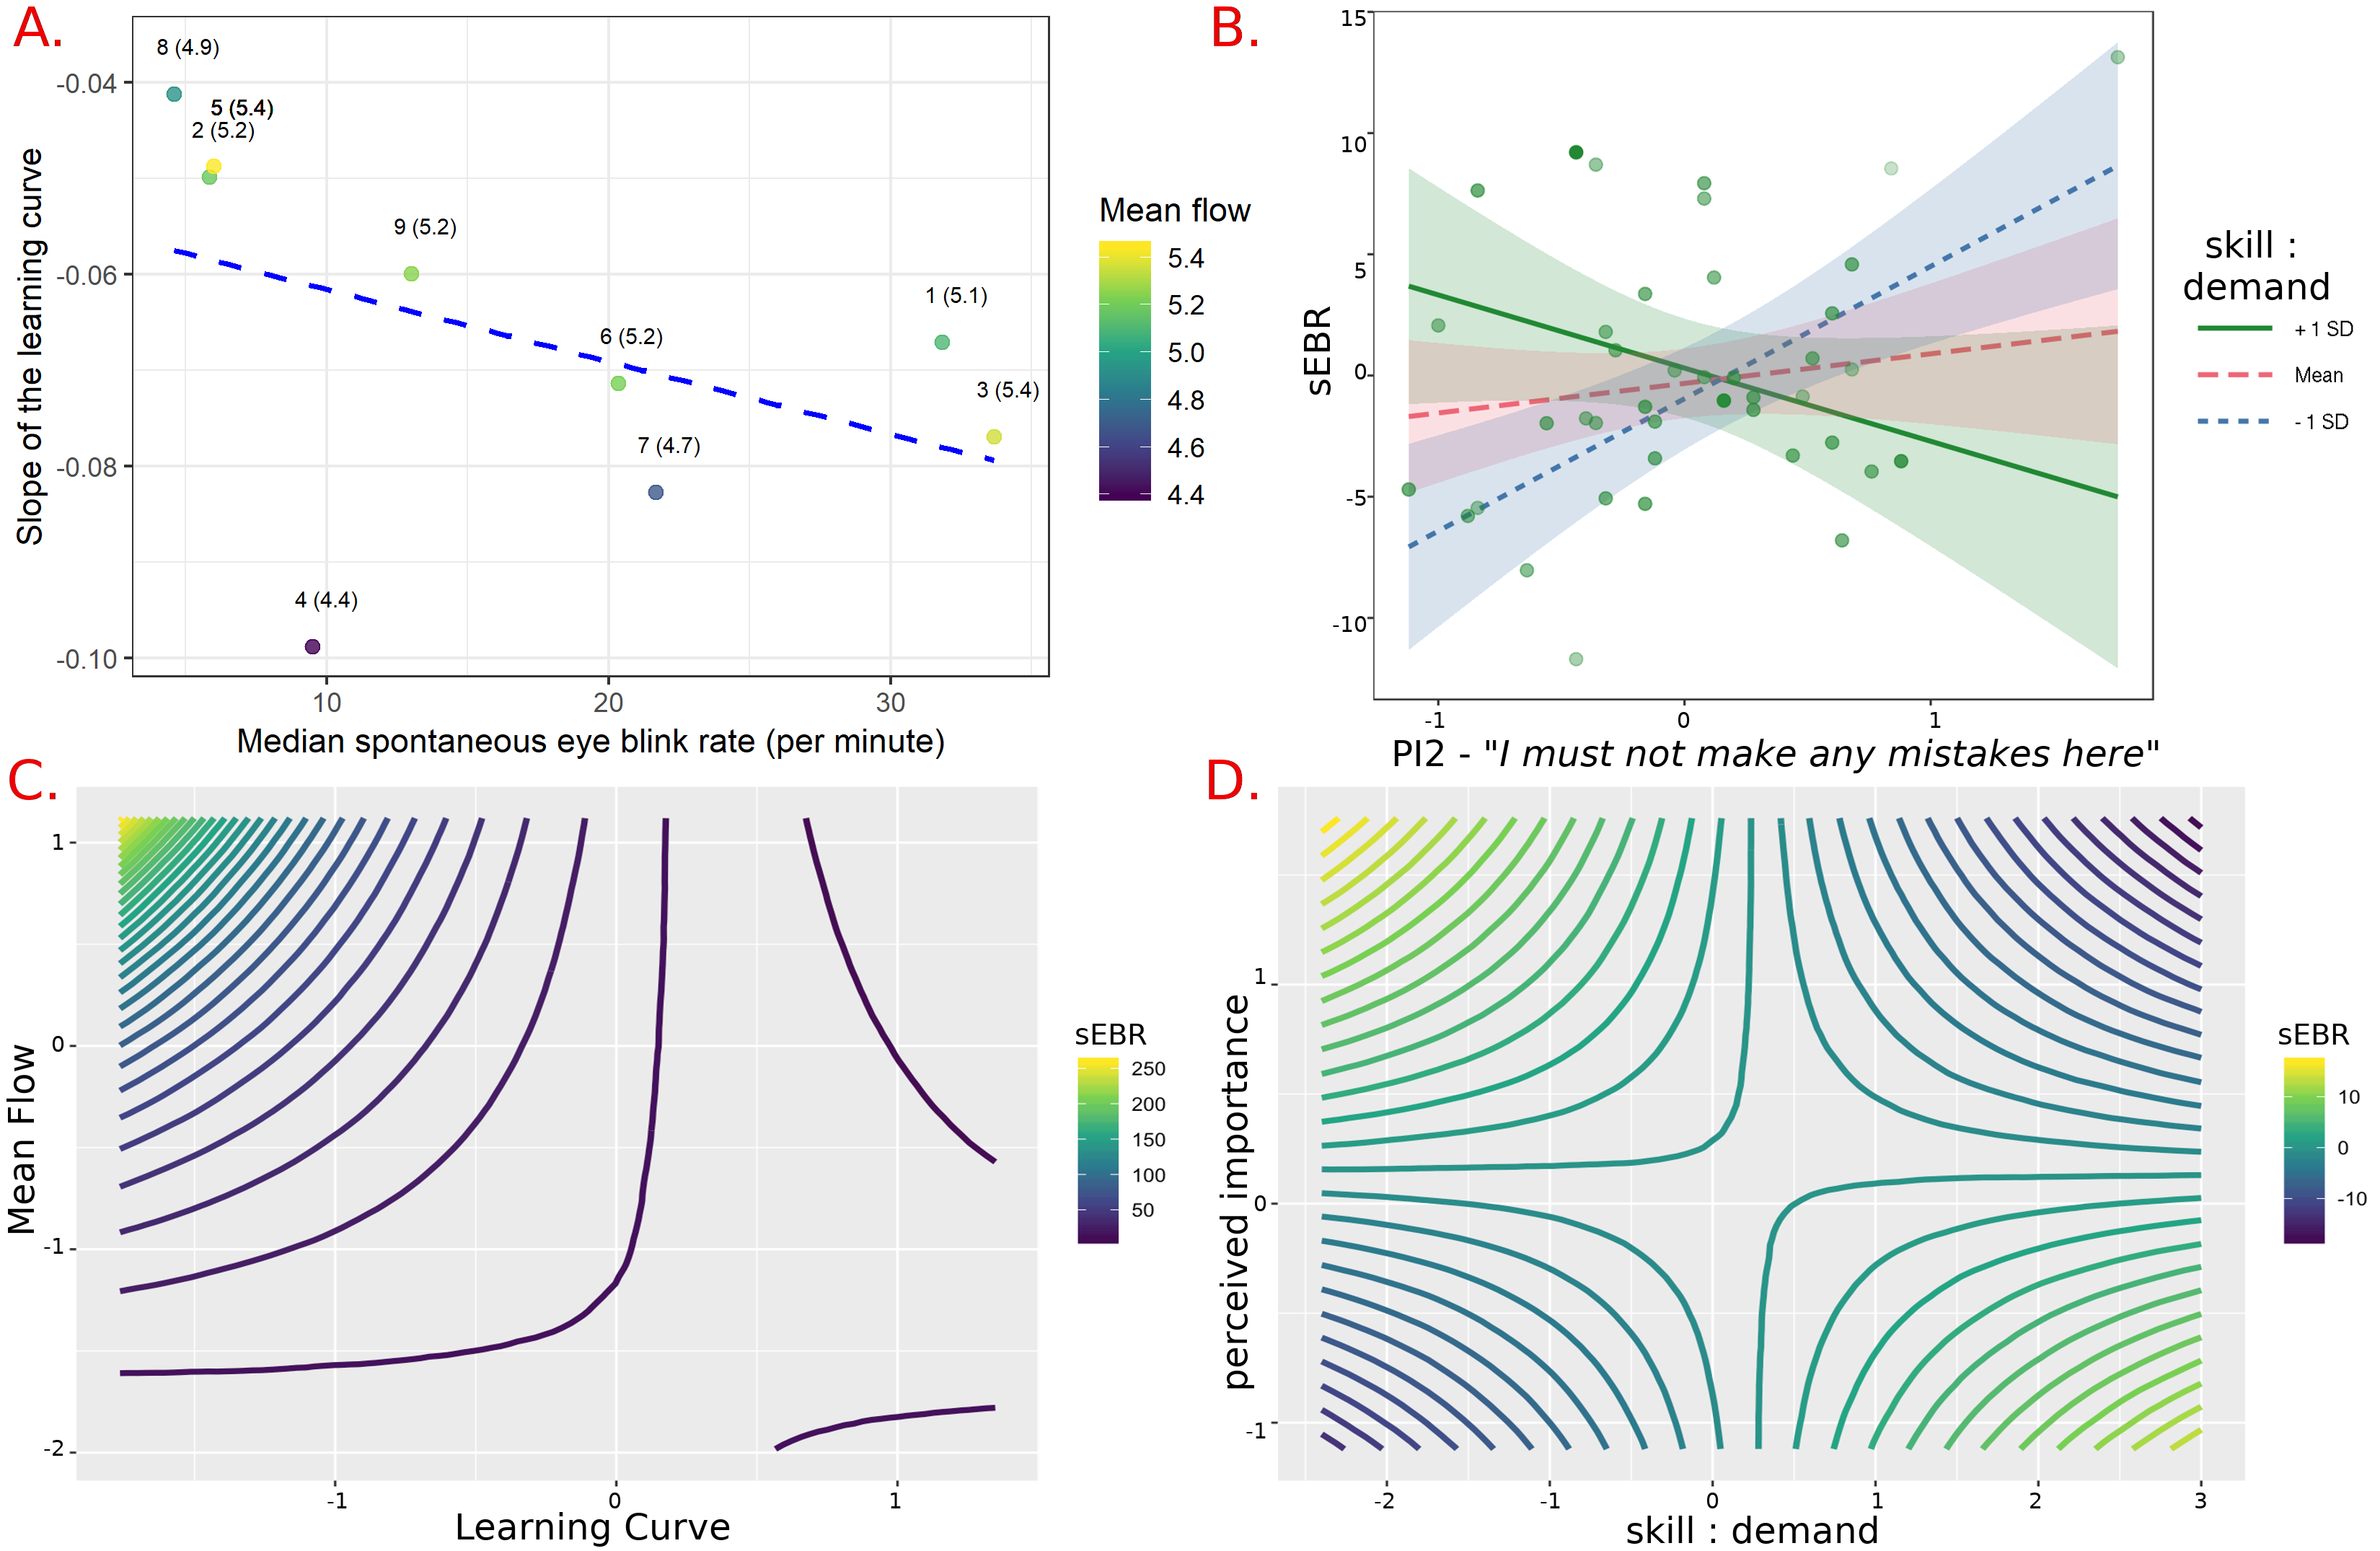
\includegraphics[width=\textwidth]{sEBR_RQ1-2_results}
	\caption{Results. \textbf{Panel A}: Participants' median sEBR plotted against their LC slope, and coloured by mean Flow scores (\textit{Note} all slopes are negative, so smaller slope = shallower LC). Linear model is depicted by the dashed line. Each point is labelled with participant number (1..9) and mean Flow (in parentheses). \textbf{Panel B}: Interaction plot for session-wise skill-demand$\times$PI.2 LMM; lines are linear models fitted at fixed levels of skill-demand. \textbf{Panel C}: Marginal effects of Bayesian model for participant-wise Flow$\times$LC. \textbf{Panel D:} Marginal effects of Bayesian model for session-wise skill-demand$\times$PI.2.}
	\label{fig:EBRvLC}
\end{figure*}


\begin{table}[!hb]
\centering
\caption{Outcome of simple-slopes analysis; \textbf{above}: for participant-wise Flow$\times$LC interaction; \textbf{below} for session-wise skill-demand$\times$PI.2 interaction.}
\begin{tabular}{llllll}
\hline
Level  & Flow & Est.     & S.E.   & \textit{t} & \textit{p} \\
\hline
+ 1 SD & 5.40 & -1096.31 & 221.36 & -4.95 & 0.0001 \\
Mean   & 5.06 &  -683.33 & 143.15 & -4.77 & 0.0001 \\
- 1 SD & 4.73 &  -270.35 & 158.23 & -1.71 & 0.6 \\
\hline
       & Skill- &      &      &            & \\
Level  & demand & Est. & S.E. & \textit{t} & \textit{p} \\
\hline
+ 1 SD & 0.96 &    -3.02 &   1.91 & -1.58 & 0.6 \\
Mean   &-0.04 &     1.22 &   1.24 &  0.99 & 0.66 \\
- 1 SD &-1.04 &     5.46 &   1.43 &  3.81 & 0.0001 \\
\hline
\label{tab:simpslopes}
\end{tabular}
\end{table}

\noindent\textbf{RQ2: session-wise sEBR and self-report}\quad
LOO testing of Bayesian models showed best out-of-sample predictive accuracy for the interaction of skill-demand and PI.2 (``\textit{I must not make any mistakes here}''/error aversion). Visual diagnostics (created as above) indicated acceptable fit for the posterior predictive distribution. Model diagnostics (Eff.Sample = 4369 and Rhat = 1.0) indicate acceptable level of convergence. For this model, 95\% HDI of the posterior sample distribution is -6.41..-1.83, so the interaction effect is non-zero. 

LMM for skill-demand$\times$PI.2 predicting sEBR showed the interaction was significant (df = 37, t = -3.680, p $<$ 0.01). %NHST7
Fig.~\ref{fig:EBRvLC} panel D shows the interaction at fixed levels of skill-demand (created by \verb|jtools::interact_plot|). SSI analysis shows that when demand exceeds skill, the PI.2 slope significantly predicts sEBR at {\it p} $<$ 0.0001. %NHST10
Fig~\ref{fig:EBRvLC}, panel D, shows how the Bayesian model of interaction (made by \verb|brms::marginal_effects|) extends insight beyond SSI.

%%%%%%%%%%%%%%%%%%%%%%%%%%%%%%%%%%%%%%%%%%%%%%%%%%%%%%%%%%%%%%%%%%%%%%%%%%%%%%%%
%%%%%%%%%%%%%%%%%%%%%%%%%%%%%%%%%%%%%%%%%%%%%%%%%%%%%%%%%%%%%%%%%%%%%%%%%%%%%%%%
%%%%%%%%%%%%%%%%%%%%%%%%     DISCUSSION    %%%%%%%%%%%%%%%%%%%%%%%%%%%%%%%%%%%%%
\section{Discussion}
For RQ1, we report evidence that LC slope is predicted by the participants' sEBR, moderated by mean Flow. This potentially indicates a role for striatal dopamine in learning the visuomotor steering task, in interaction with subjective experience. 
Regarding RQ2, we found a dissociation between PI.2 (error aversion) and skill:demand balance depending on sEBR level. \textbf{In other words}: for high sEBR participants, skill$>$demand $\rightarrow$ low error aversion and \textit{vice versa}; for low sEBR participants, skill$>$demand $\rightarrow$ high error aversion and \textit{vice versa}.

Given the reinforcement-learning nature of our task (positive reinforcement from speed increase, negative reinforcement from collisions), what do these results tell us?

% Relation to previous Work on eye blink rate
% \paragraph{RQ1 - Learning, Flow, and sEBR:}
% Evidence for RQ1 suggests a clear linear trend relating sEBR and LCs (Fig.~\ref{fig:EBRvLC}): the larger the sEBR, the steeper the LC slope (or: the higher the LC intercept). The distance of data-points from the fitted model values also closely match the distribution of Flow mean scores, meaning that individuals with lowest Flow also diverge the most from the sEBR$\times$LC model. Interaction analysis then supports the idea that sEBR correlation with LC is stronger the higher the mean Flow. We thus claim that there is a genuine sEBR--LC relationship that is moderated by Flow.

The caudate nucleus of the striatum plays a major role in decision making and reward/aversion processing \citep{Slagter2015}. It is moderated by tonic dopamine D2-receptor level, which can thus bias the entire learning process; indeed predisposition for Flow was shown to be positively correlated with striatal dopamine D2-receptor availability \citep{DeManzano2013}. One mechanism for this is illustrated in a study of `attentional blink' (AB) by \citet{Slagter2012}, which suggest a U-shaped function between tonic striatal dopamine and AB size. In other words, very high or low levels of dopamine D2-receptor density can make attention updating too rapid (distractable) or too slow (inattentive).

% \hl{Let us consider learning as a process whereby perception, cognition and action become attuned to task demands.} 

In our game task, learning involves high-frequency decision making with respect to continuously updating stimuli of uniform kind (not unlike the AB-probe task of \citet{Slagter2012}). In this view, RQ1 could be interpreted as showing that higher D2 density indexed by sEBR facilitates learning, with greater effect for those who were predisposed to experience Flow. 
% An alternative interpretation is that it reflects higher distractability in the early phases of learning (LC intercept).
% greater ease of getting into Flow, becoming attuned to the task, and thus learning 
The underlying mechanism could be that higher dopamine levels permit more rapid attention updating and thus more fluid response to changing task demands. In the context of this study, this hypothesis can work despite \citet{Slagter2012}'s proposed U-shaped function: because our game-task constantly maintains a level of demand slightly greater than the participants' skill, and the {\it requirement} for rapid attention updating grows with learning. Thus, in this context, higher median sEBR tends to be better, \textit{if more Flow is experienced}. Lower Flow could be due to, e.g., misalignment of task demands and attentional updating rate, creating a more effortful experience.

% \hl{So the observed moderation by Flow scores of the sEBR--LC relationship could be speculated to have a basis in adjusting attention updating, in response to changing task speeds, physiologically underpinned by the nigro-striatal DA system.} 
In other words, it may not be the case that an absolute level of striatal dopamine should predict learning, but rather an individual level relative to how each participant relates to the task. If a participant's tonic dopamine is not at their ideal level for this task, they might nevertheless do well in the task, and yet find the experience more effortful and less fluid.
% (than is suggested as Flow-like by wording of the FSS).

The RQ2 dissociation result, which accounts for variation across sessions as well as between participants, indicates how sEBR can signify differences in error aversion under different subjective conditions of skill:demand balance.

%%%%%%%%%%%%%%%%%%%%% POST-HOC MATERIAL OF VITAL IMPORTANCE %%%%%%%%%%%%%%%%%%%%


\section{Acknowledgements}
We thank Otto Lappi, Kalle Toikka, and Juha Veps\"{a}l\"{a}inen.


\bibliographystyle{apacite}

\setlength{\bibleftmargin}{.125in}
\setlength{\bibindent}{-\bibleftmargin}

\bibliography{CogCarFlow_bib}

\end{document}
